\documentclass{acm_proc_article-sp}

\usepackage{amsmath}

% algorithm
\usepackage{algorithmicx}
\usepackage{algorithm}% http://ctan.org/pkg/algorithms
\usepackage[noend]{algpseudocode}% http://ctan.org/pkg/algorithmicx

\begin{document}

\title{A Novel Similarity-Search method for Mathematical \\ Content in {\ttlit LaTeX} Markup}

\numberofauthors{2} 
\author{
\alignauthor Wei Zhong,\; Hui Fang\\
       \affaddr{Dept. of Electrical and Computer Engineering}\\
       \affaddr{University of Delaware}\\
       \affaddr{Newark, DE USA}\\
       \email{\{zhongwei, hfang\}@udel.edu}
}

\maketitle
\begin{abstract}
A relaxed structural matching search method, along with a symbolic similarity measurement algorithm for mathematical content search is proposed. 
Our approach uses an intermediate tree representation to capture structural information of mathematical expression, and based on a previous idea which indexes math expression structure through tree leaf-root paths, we further describe an advanced AND search method in a formal way. This search method can be used to test query/document subexpression isomorphism or evaluate the symbolic similarity between math expressions with consideration of their $\alpha$-equivalence. 
For the purpose of evaluation, we also implement a search engine based on our idea. 
\end{abstract}

\category{H.3}{Information Search and Retrieval}{Miscellaneous}
\terms{Algorithms}

\keywords{mathematical searching, language processing, search engine}

\section{Introduction}
\label{intro}
With \textit{MathJax} becoming popular, more and more \LaTeX{} markup can be crawled directly from many websites. 
In order to search those mathematical language in \LaTeX{} markup, a search method that can respect the properties of math expression needs to be developed. 
Although many researches have been conducted to retrieve information in structured content (e.g. \textit{MathML}), information retrieval on \LaTeX{} math content is still not well-studied or exhaustively covered by mainstream IR research, compared to that on general text.

Unlike general text content, mathematical language, by its nature, has many differences from other textual documents, there are a number of new problems in measuring mathematical expression similarity.
Among those problems, we know one math expression can be transformed to alternative forms, e.g. $\frac{a + b}{c}$ and $\frac{a}{c} + \frac{b}{c}$ should be considered as semantically identical. To identify those variations requires search engine to apply mathematical transformation rules to a query in order to obtain all forms of relevant expressions. 
Further, math expressions with the same evaluated value may also be considered relevant, in this case, $\sin(\frac {\pi} 2)$ and $1$ are equivalent. Some computational search engines (e.g. \textit{Symbolab} and \textit{WolframAlpha}) are aware of these problems.
But sometimes we need to rely on conventions and context to distinguish expressions such as $f(a+b)$ and $c(a+b)$, because the symbol $f$ in the former expression is likely to represent function instead of a variable, 
in addition, expression such as $f^{-1}$ can either be reciprocal or an inverse function.
Moreover, a higher level of understanding of mathematic knowledge may be required for math-aware search engine to find the results for queries such as ``find an article related to the four color theorem" (from NTCIR-10 Math topics~\cite{ntcirtopic}).

Yet the problems addressed above are not considered in this paper, instead, we are focusing on the aspects which does not require a ``good understanding" of mathematics, we target our research domain to be the following:
The first is structural similarity. For example, $ax+(b+c)$ is not equivalent to $(a+b)x+c$ although they have the same set of symbols, this is because their structural difference. However, as the position of operands in math expression can be commutative in some cases, structural similarity is often measured by substructure isomorphism if we use operation tree~\cite{goodsurvey} to represent math expressions.
The second is symbolic similarity, with the consideration of $\alpha$-equivalence. We know that symbols can be used interchangeably in each math formula to express the same meaning, e.g. $a^2+b^2=c^2$ and $x^2+y^2=z^2$. Nevertheless, we still weight symbolic similarity sometimes, for instance, $E=mc^2$ is considered more meaningful when exact symbols are used rather than just being structurally identical with $y=ax^2$.
On the other hand, we should also weight $\alpha$-equivalent expressions more, that is, changes of symbols in expression preserve more syntactic similarity when changes are made by substitution, e.g. for query $x(1+x)$, expression $a(1+a)$ are considered more relevant than $a(1+b)$. Because the ``bond variable" $x$ and $a$ here are at the same positions and both supposed to represent the same value.
All the points addressed here makes transitional IR methods (e.g. bag of words model and tf-idf weighting) deficient to handle math content. 

\section{Related Work}
Similarity/boolean search for mathematical content is not a new topic,
conference in this topic is getting increasingly research attention and the proposed systems have progressed considerably~\cite{ov}.
DLMF project from NIST~\cite{Youssef03,Youssef05} and MIaS system~\cite{mias11a,mias11,mias:thesis}, notably, use text-based approaches and utilize existing models to deal with math content on top of existing IR tools (such as \textit{Apache Lucene}). 
They are commonly using augmentation and normalization (by ordering the subexpressions) to enumerate and represent all possible sequences of commutative operands (symbols (e.g. $a$ and $b$) and unified items (\textit{id}, \textit{const}) in different levels of math expression.
MWS~\cite{Kohlhase06,Kohlhase0p4,Kohlhase0p5} takes a \textit{automatic theorem proving} approach and uses \textit{term indexing}~\cite{graf96} to minimize the cost of unification algorithm which is able to find if two expressions are equivalent, 
however, their index relies on RAM memory~\cite{Kohlhase0p5} and needs to include all sub-terms of a formula~\cite{Kohlhase06}.
A \textit{symbol layout tree} or \textit{presentation tree}~\cite{symbollayout12,WikiMirs13} is introduced to describe geometric layouts of symbols in a formula. 
\cite{WikiMirs13} uses two templates to parse \LaTeX\ markup with two typical operator terms: explicit ones (``\textbackslash frac", ``\textbackslash sqrt", etc.) and implicit ones (``$+$", ``$\div$", etc.) to form a presentation tree,
then extracts original terms and generalized terms from normalized presentation tree, to provide the flexibility of both fuzzy and exact search.
\cite{symbollayout12} uses symbol layout tree as a kind of substitution tree, while \cite{symbolpairs15,symbolpair15:2} have developed a \textit{symbol pairs} idea to capture relative position information between symbol pairs,
which enables key-value storage to speed search.
\cite{newretrievalsystem} extracts HASH signature for each subtree, their system has a slower index growth resulted from a lot of occurrences of common subtree structure in math expressions.
\cite{DOMextraction} extracts semantic keywords, structure description to indicate subordinative relationship in a string format. The similarity is calculated using normalized tf-idf vector.
Tree edit distance is adopted by \cite{editdisXML11,editdisXML13} in which they try to overcome the bad time complexity of original algorithm by summarizing and using a compromised edit distance algorithm, then by applying with an early termination algorithm along with a distance cache.
There are also efforts using image-based approaches~\cite{imageb11,handwrite} and lattice-based approach~\cite{lattice} to measure math formula similarity in a different perspective.

\section{Methodology}
\begin{figure}
\begin{minipage}[b]{1.60in}
\begin{center}
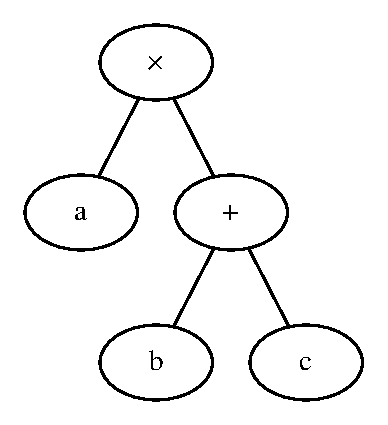
\epsfig{height=1.3in,width=1.0in,file=res/leafroottree.eps}
\\$a(b+c)$ in operation tree
\end{center}
\end{minipage}
\hspace*{0in}
\begin{minipage}[b]{1.60in}
\begin{center}
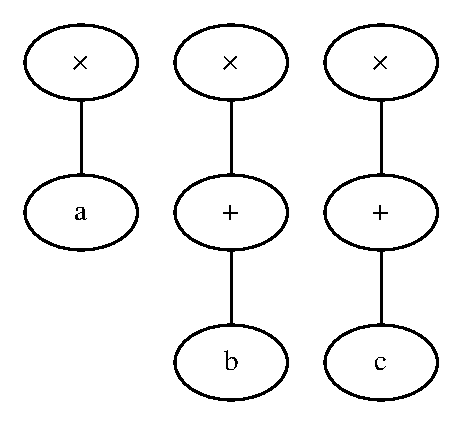
\epsfig{height=1.3in,width=1.2in,file=res/leafrootpath.eps}
Generated leaf-root paths
\end{center}
\end{minipage}
\caption{Leaf-root path example}\label{oprtreeExample}
\end{figure}
Our method can be seen as an approach built upon the idea of leaf-root path or sub-path~\cite{signifjap,MathMLleafroot,signfused,sefobyfo} from an operation tree, to capture structure and semantic information of math expression. 
Figure~\ref{oprtreeExample} is an example of generated leaf-root paths for math expression $a(b+c)$.
The intuition behind this idea is that an operation tree, no matter how operands are ordered, uniquely determines the leaf-node paths decomposed from the tree.
This makes leaf-root path a good fit for representing mathematical expression because commutative operands are exhaustively used in mathematical language.
Besides, by going bottom-up from leaves of an operation tree, we are essentially traversing to an expression from its subexpression for every level. 
So we can index the leaf-root paths and search an expression by going through and beyond the leaf-root paths from its subexpression.

We develop these ideas to simultaneously search along the way of all leaf-root paths, so that we are essentially pruning indexes which does not share the common postfixes beyond the root of the query tree.
To better describe further ideas build upon this, we will put it in a formal way.

\subsection{Formal Definition}
Here we clarify some notations used throughout this paper, a path $p$ is a sequence of numbers given by $p = p_0 p_1 \ldots p_n,\; n\ge0$, $p_i \in \mathbf{R}$ and $\mathbf{P}$ is the set of all paths.
Any function $f(\cdot) = y \in \mathbf{R}$ applied on path $p$ is mapped to a path too: $f(p)=f(p_0)f(p_1) \ldots f(p_n)$.
And we name  a \textit{concatenation} of two paths $\,^1p = p_0p_1 \ldots p_n$ and $\,^2p = p_np_{n+1} \ldots p_m$ where $m \ge n$, to be a new path $\,^1p \cdot \,^2p$ defined as $p_0p_1 \ldots p_n p_{n+1} \ldots p_m$,
and the concatenation of a path $p$ on a set $S = \{ s_1, s_2 \ldots s_n \}$ is defined as $S \cdot p = \{ s_1\cdot p,\  s_2\cdot p \ \ldots \ s_n\cdot p \}$.
A path with only one element can be explicitly wrapped by a bracket, e.g. $p=(p_0)$, to avoid confusion.
Furthermore, \textit{the longest common postfix} path $p^*$ between two path $p_1$ and $p_2$ is mapped by the function named $\mathrm{lcp}$, which is defined by $p^* = \mathrm{lcp}(p_1, p_2) = \mathrm{lcp}(p_2, p_1)$.

We introduce a \textit{formula tree} to represent a mathematical expression, in which each node is associated with a label to represent the unified token (e.g. same value for token $+$, $\oplus$ and $\pm$) and each leaf node is associated with a symbol to identify math expression operand. 
Besides, a \textit{formula subtree} relation is also defined to address the sub-structure relation between two mathematical expressions.

\subsubsection{Formula tree}
A \textit{formula tree} is a labeled rooted tree $T = T(V,E,r)$ with root $r$, where each vertices $v \in V(T)$ is associated with a label (not necessarily unique in the same tree) $\ell_T(v) \in \mathbf{R}$ mapped by label function $\ell_T$,
and each leaf $l \in V(T)$ is also associated with a symbol $\mathcal{S}_T(v) \in \mathbf{R}$ mapped by symbol function $\mathcal{S}_T$. For convenience, we will write $\ell$ and $\mathcal{S}$ as short names which refer to the tree implied by the context, also we use function $\mathcal{S}(p)$ to indicate the symbol of the leaf in a leaf-root path $p$.

\subsubsection{Formula subtree}
\label{frmlsubtreeDef}
Given formula tree $S$ and $T$, we say $S$ is a \textit{formula subtree} of $T$ if there exists an injective mapping $\phi: V(S) \rightarrow V(T)$ satisfying:

\begin{enumerate}
\item 
$\forall\; (v_1,v_2) \in E(S)$, we have $(\phi(v_1),\phi(v_2)) \in E(T)$;
\item
$\forall\; v \in V(S)$, we have $\ell(v) = \ell(\phi(v))$;
\item
If $v \in V(S)$ is a leaf vertices in $S$, then $\phi(v)$ is also a leaf in $T$.
\end{enumerate}
Such a mapping $\phi$ is called a formula subtree isomorphic embedding (or formula embedding) for $S \rightarrow T$. 
If satisfied, we denote $S \preceq_l T$ on $\Phi$, where $\Phi$ ($\Phi \neq \emptyset$) is the set of all the possible formula embeddings for $S \rightarrow T$.

\subsubsection{Leaf-root path set}
A \textit{leaf-root path set} generated by tree $T$ is a set of all the leaf-root paths from tree $T$, mapped by a function $g(T)$. 

\subsubsection{Index}
An \textit{index} $\Pi$ is a set of trees such that $\forall\; T \in \Pi$, we have $T \in \mathcal{I}_{\Pi}(a)$ for any $a \in \ell(g(T))$, we say $T$ is indexed in $\Pi$ and $\mathcal{I}_{\Pi}$ is called an index look-up function for index $\Pi$. 

\subsection{Search Method}
For a collection of document expressions, we will index them by merging all the leaf-root paths from each document formula tree into a large ``inverted" index tree, 
in which each node from path $a$ stores the information of all the indexed formula trees in $\mathcal{I}_{\Pi}(a)$.

Through searching all sub-paths at the same time, we are able to limit the set of formula trees being structurally matching (in formula subtree relation) with a query formula tree, to only a subset of our index. 
This is illustrated as follows.

Given an index $\Pi$ and a formula tree $T_q$, $\forall\; T_d \in \Pi$:
If $T_q \preceq_l T_d$ on $\Phi$, then $\exists\; \hat{a} \in \mathbf{P},\; s.t.$
$$
T_d \in \bigcap_{a \in L} \mathcal{I}_{\Pi}(a)
$$
where $L = \ell(g(T_q)) \cdot \hat{a}$.

\textit{Justification.}
Denote the root of $T_q$ and $T_d$ as $r$ and $s$ respectively.
Let $\hat{p}$ be the path determined by vertices from $t=\phi(r)$ to $s$ in $T_d$,
and $\,^1p, \,^2p \ldots \,^np,\; n \ge 1$ be all the leaf-node paths in $T_q$.
Then $\hat{a} = \ell(\hat{p})$, this is because:
$L = \ell(\{ \,^1p, \,^2p \ldots \,^np \}) \cdot \hat{a} = 
\ell(\{ \phi(\,^1p), \phi(\,^2p) \ldots \phi(\,^np) \}) \cdot \ell(\hat{p}) =
\{ \ell(\phi(\,^1p) \cdot \hat{p}), \ell(\phi(\,^2p) \cdot \hat{p}) \ldots \ell(\phi(\,^np) \cdot \hat{p}) \}
$.
According to definition~\ref{frmlsubtreeDef} and $t=\phi(r)$, we have $\phi(\,^ip) \cdot \hat{p} \in g(T_d),\; 1 \le i \le n$.
Since $ T_d \in \Pi$, $T_d$ is indexed in $\Pi$ with respect to each of the elements in $L$, that is to say $\forall\; a \in L, \; T_d \in \mathcal{I}_{\Pi}(a)$.

\begin{figure}
\begin{minipage}[b]{1.65in}
\begin{center}
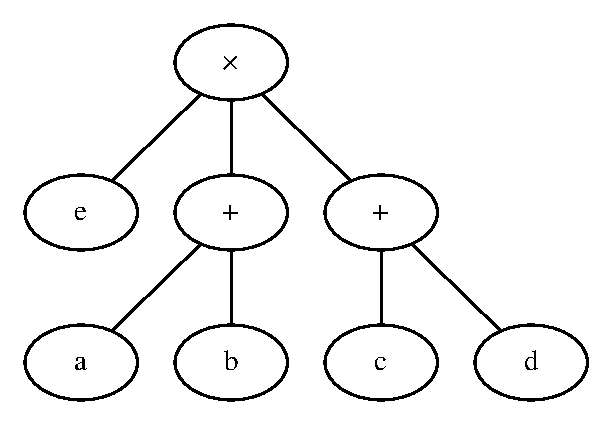
\epsfig{height=1.3in,width=1.6in,file=res/not-necessary.eps}
\\ $(a+b) \times (c+d) \times e$
\end{center}
\end{minipage}
\hspace*{.0in}
\begin{minipage}[b]{1.60in}
\begin{center}
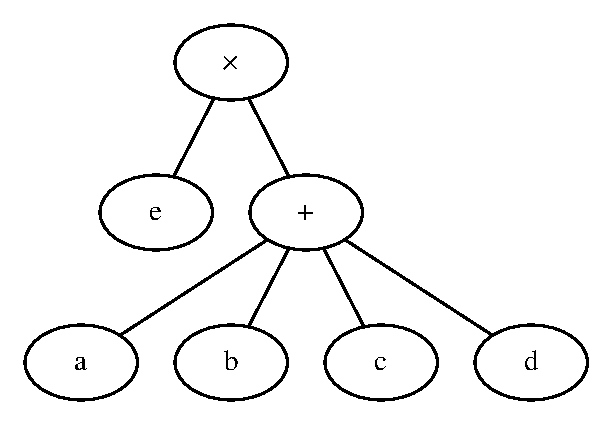
\epsfig{height=1.3in,width=1.5in,file=res/not-necessary2.eps}
\\ $(a+b+c+d) \times e$
\end{center}
\end{minipage}
\caption{Leaf-root paths with different structure}\label{notnecessary}
\end{figure}

In a nutshell, we search the index by intersecting the indexed formula trees from all the generated leaf-node paths at the same time, then further possible search path $\hat{a}$ is only possible when paths along the generated leaf-node paths in the index have a common postfix.
Therefore we can ``merge" the paths ahead and prune those paths not in common. Level by level, we are always able to find the structurally matched formula tree as long as it is indexed in $\Pi$.

\subsection{Substructure Matching}
However, query formula tree will not necessarily being formula subtree to all the document (indexed) formula trees in our search set
$\bigcap_{a \in L} \mathcal{I}_{\Pi}(a)$,
even if their generated leaf-root paths are identical.
One supporting example for this point is shown in figure~\ref{notnecessary}.
To address this problem, we propose an algorithm described in in figure~\ref{submatchalgo}, to test the document formula trees in our search set to see if they are in formula subtree relation.
This algorithm is inspired from the following observations. 

\begin{figure}
\begin{algorithmic}[1]

\Procedure{removeCandidate}{$d,Q,C$}
\For {$a \in Q$}
\If{$C_a = \emptyset$}
\State \textbf{return} $\emptyset$
\Else
\State {$C_a := C_a - \{d\}$}
\EndIf
\EndFor
\State \textbf{return} $C$
\EndProcedure

\State {}

\Procedure{match}{$a, a', Q, C$}
\For {$b \in Q$}
\State $t := \mathrm{lcp}(a,b)$
\State $Q_t := Q_t \cup \{b\}$
\State $P := P \cup \{t\}$
\EndFor
\For {$t \in P$}
\For {$b \in Q_t$}
\For {$b' \in C_b$}
\If {$t \not= \mathrm{lcp}(a',b')$}
\State $C := $ \Call{removeCandidate}{$b', Q_t, C$}
\If {$|C| = 0$}
\State \textbf{return} FAIL
\EndIf
\EndIf
\EndFor
\EndFor
\If {\Call{decomposeAndMatch}{$Q_t, C$} = FAIL}
\State \textbf{return} FAIL
\EndIf
\EndFor
\State \textbf{return} SUCC
\EndProcedure

\State {}

\Procedure{decomposeAndMatch}{$Q, C$}
\If {$Q = \emptyset$} \textbf{return} SUCC
\EndIf
\State $a$ := OnePathIn(Q)
\Comment{Choose a reference path in Q}
\State $Q_{\mathrm{new}} := Q - \{a\}$
\For {$a' \in C_a$}
\State $C_{\mathrm{new}} := $ \Call{removeCandidate}{$a', Q_{\mathrm{new}}, C$}
\If {$C_{\mathrm{new}} = \emptyset$} \textbf{return} FAIL
\EndIf
\If {\Call{match}{$a, a', Q_{\mathrm{new}}, C_{\mathrm{new}}$}}
\textbf{return} SUCC
\EndIf
\EndFor
\State \textbf{return} FAIL
\EndProcedure

\end{algorithmic}
\caption{The decompose-and-match algorithm}\label{submatchalgo}
\end{figure}

\subsubsection{Observation 1} 
\label{observation1}
For two formula trees which satisfy $T_q \preceq_l T_d$ on $\Phi$, then $\forall\; \phi \in \Phi,\, p \in g(T_q)$, also any vertices $v$ along path $p$, the following properties are obtained:
\begin{eqnarray}
\deg(v) \le \deg(\phi(v)) \label{prop1} \\
\ell(p) = \ell(\phi(p)) \label{prop3} \\
\left| g(T_q) \right| \le \left| g(T_d) \right| \label{prop4}
\end{eqnarray}
\textit{Justification.} 
Because $\forall\; w \in V(T_q) \  s.t. \  (v, w) \in E(T_q)$, there exists $(\phi(v), \phi(w)) \in E(T_d)$. 
And for any (if exists) two different edges $(v, w_1), (v, w_2) \in E(T_q),\, w_1 \not= w_2 \in V(T_q) $, we know $(\phi(v), \phi(w_1)) \not= (\phi(v), \phi(w_2))$ by definition~\ref{frmlsubtreeDef}. 
Therefore any different edge from $v$ is associated with a distinct edge from $\phi(v)$, thus we can get (\ref{prop1}). 
Given the fact that every non-empty path $p$ can be decomposed into a series of edges $(p_0, p_1), (p_1, p_2) \ldots (p_{n-1}, p_n), \; n > 0$,
property (\ref{prop3}) is trivial.
Because there is exact one path between every two nodes in a tree, the leaf-root path is uniquely determined by a leaf node in a tree. Hence the rationale of (\ref{prop4}) can be obtained in a similar manner with that of (\ref{prop1}), expect neighbor edges are replaced by leaf-node paths.


\subsubsection{Observation 2} 
\label{observation2}
Given two formula trees $T_q$ and $T_d$, if $\left| g(T_q) \right| = 1$ and $\ell(g(T_{q})) \subseteq \ell(g(T_d))$, then $T_q \preceq_l T_d$.

\noindent \textit{Justification.} 
Obviously there is only single one leaf-root path in $T_q$ because $\left| g(T_q) \right| = 1$. 
Denote the path as $p = p_0 \ldots p_n,\; n \ge 0$ where $p_n$ is the leaf, and let $a = \ell(p)$.
Since $a \subseteq \ell(g(T_d))$, we know that there must exist a path $p'=p'_0 \ldots p'_n \in g(T_d)$ such that $a = \ell(p')$.
Without loss of generality, suppose $p'_n$ is the leaf of $T_d$. 
Now the injective function $\phi: p_i \rightarrow p'_i,\  0 \le i \le n$ satisfies all the requirements for $T_q$ as a formula subtree of $T_d$.

\subsubsection{Observation 3} 
\label{observation3}
For two formula trees $T_q$ and $T_d$, if $T_q = T(V,E,r) \preceq_l T_d$ on $\Phi$,  
$\forall a,b \in g(T_q)$ and a mapping $\phi \in \Phi$. 
Let $T_d' = \, ^{t}T_d$ where $t = \phi(r)$ and $a' = \phi(a)$, $\forall\; b' \in g(T_d')$, it follows that:
$$
\begin{array}{lcr}
b' = \phi(b)  & \Rightarrow & 
\left| \mathrm{lcp}(a,b) \right| = \left| \mathrm{lcp}(a',b') \right|
\end{array}
$$
Furthermore, $\forall\; c \in g(T_q)\; s.t.\; \left| \mathrm{lcp}(a,b) \right| \neq \left| \mathrm{lcp}(a,c) \right| $, we have
$$
\begin{array}{lcr}
\left| \mathrm{lcp}(a,b) \right| = \left| \mathrm{lcp}(a',b') \right|
& \Rightarrow &
b' \neq \phi(c)
\end{array} 
$$
\textit{Justification.} 
Because $a,b \in g(T_q)$, thus $a_0 = b_0 = r$, and we can also make sure $\mathrm{lcp}(a,b) \ge 1$. 
Denote the path of $a = a_0 \ldots a_n a_{n+1} \ldots a_{l-1}$, similarly denote the path of $b$ as $b=b_0 \ldots b_n b_{n+1} \ldots b_{m-1}$,
where the length of each $l,m \ge 1$ and $a_i = b_i,\, 0 \le i \le n \le \min(l-1, m-1)$ while $a_{n+1} \neq b_{n+1}$ if $l,m > 1$.
On the other hand $a' = \phi(a)$ and $b' \in g(\,^{t}T_d)$, therefore $a'_0 = \phi(a_0) = \phi(r) = t = b'_0$.
For the first conclusion, if $b' = \phi(b)$, there are two cases. If any of $|a|$ or $|b|$ is equal to one then $\left| \mathrm{lcp}(a,b) \right| = |(r)| = |(t)| = \left| \mathrm{lcp}(a',b') \right| = 1$;
Otherwise if $l,m > 1$, path $a_0 \ldots a_n = b_0 \ldots b_n$ and $a_{n+1} \neq b_{n+1}$ follow that $\phi(a_0 \ldots a_n) = \phi(b_0 \ldots b_n)$ and $\phi(a_{n+1}) \neq \phi(b_{n+1})$ by definition.
Because edge $(\phi(a_n), \phi(a_{n+1}))$ and $(\phi(b_n), \phi(b_{n+1}))$ are also in $E(T'_d)$, 
we have $\left| \mathrm{lcp}(a,b) \right| = \left| \mathrm{lcp}(a',b') \right| = n$.
For the second conclusion, we prove by contradiction. 
Assume $b' = \phi(c)$, by the first conclusion we know $\left| \mathrm{lcp}(a,c) \right| = \left| \mathrm{lcp}(a',b') \right|$.
On the other hand, because $\left| \mathrm{lcp}(a,c) \right| \neq \left| \mathrm{lcp}(a,b) \right| =  \left| \mathrm{lcp}(a',b') \right|$, 
thus $\left| \mathrm{lcp}(a,c) \right| \neq \left| \mathrm{lcp}(a',b') \right|$ which is impossible. 

For a query formula tree $T_q$ and a document formula tree $T_d$, observation 1 offers us some constrains for finding initial possible isomorphic paths in $T_d$ (what we call \textit{candidates}) for a given query path in $T_q$.
And observation 2 is a sufficient condition to test substructure relation, but the query tree has to consist only one leaf-root path to be tested. 
While observation 3 states two necessary conditions for one formula tree to be a formula subtree of another and implies that a group of query leaf-root paths can only be isomorphic to someones in another group of leaf-root paths in document formula tree. 
This leads to the idea to decompose the formula tree and divide the problem into subproblems by ruling out impossible candidates using observation 3, until at some point we can apply observation 2 or observe trivial cases to solve all the sub-matching problems.

\begin{figure}
\begin{minipage}[b]{1.65in}
\begin{center}
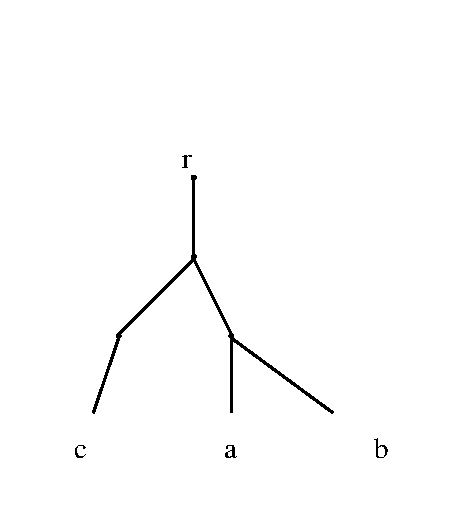
\epsfig{height=1.9in,width=1.6in,file=res/lpd.eps}
\\(a)
\end{center}
\end{minipage}
\hspace*{0in}
\begin{minipage}[b]{1.65in}
\begin{center}
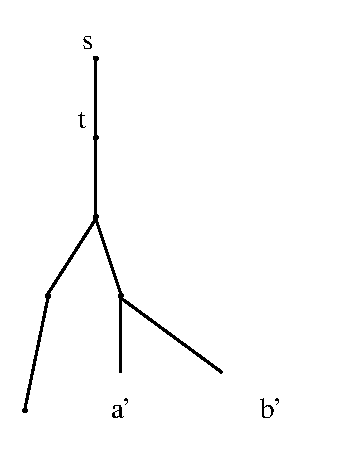
\epsfig{height=1.9in,width=1.6in,file=res/lpd2.eps}
\\(b)
\end{center}
\end{minipage}
\caption{Formula subtree matching}\label{submatch}
\end{figure}

To illustrate our \textproc{decomposeAndMatch} algorithm, figure~\ref{submatch} gives a general case in which query tree in (a) is trying to match a document tree in (b).
Initially every leaf-root path in (a) should be associated with a set of candidate paths in (b) which satisfy the constrains in \ref{observation1}.
Then we arbitrarily choose a path in (a) as a \textit{reference path} (heuristically a \textit{heavy path}~\cite{heavypathde}), for each of the paths in its candidate set, we choose it as reference path in (b), and suppose we choose $a'$ here. At this time we can apply the two constrains from \ref{observation3} and ruling out some impossible isomorphic paths in candidate set of each path in (a) and divide the problems further. 
For example, because $\left| \mathrm{lcp}(a,b) \right| = \left| \mathrm{lcp}(a',b') \right|$, we know $b'$ is still in candidate set of $b\,$; while $b'$ is not in candidate of $c$ because $\left| \mathrm{lcp}(a,b) \right| \neq \left| \mathrm{lcp}(a,c) \right|$. 
After going through these eliminations for each leaf-node path (except the reference path $a$) in (a), we now have two similar subproblems: $c$ as a subtree along with its candidate set, and $b$ as a subtree along with its candidate set. 
We can apply this algorithm recursively until a trivial subproblem is reached (e.g. the case in \ref{observation2}). During this process, if we find any candidate set to be empty, we stop the subproblem process and change to another reference path or stop the algorithm completely if every possible reference path is tried.
The argument $Q$ and $C$ is the set of leaf-root paths in query tree and the candidate sets associated with all leaf-root paths respectively.
The procedure returns \textproc{SUCC} if a matching possibility is found, otherwise \textproc{FAIL} is returned indicating the formula tree in (a) cannot not be a formula subtree of that in (b).

\textproc{decomposeAndMatch} algorithm offers a way to ``double-check" structure isomorphism, because 
for any two formula tree $T_q$ and $T_d$ and $\forall\; \hat{a} \in \mathbf{P}$, if $\ell(g(T_q)) \cdot \hat{a} \subseteq \ell(g(T_d))$, it is not sufficient to imply $T_q \preceq_l T_d$.
Nevertheless, we think the cases which makes the above statement insufficient are fairly rare in common mathematical content, and the complexity introduced from this algorithm will offset the benefit to identify the structure isomorphism.
Thus a compromised search, for efficiency reason, would assume all the document formula trees in search set
$\bigcap_{a \in L} \mathcal{I}_{\Pi}(a)$ is structurally matching the given query formula tree $T_q$.

\subsection{Structural Similarity}
After searching structurally matching document expressions in a boolean manner, we use two factors to measure their structural similarity degree. 

The first is \textit{matching depth}.
As it is addressed in \cite{mias11a}, the deeper sub-formulae in in mathematical expression will make it less important to the overall formula.
For example, given query formula $\sqrt a$, expression $\sqrt {x}$ would score higher than $\sqrt{\sqrt{x}}$ does. 
To reflect the depth where two expressions match, we define \textit{matching depth factor} $f(d)$ to be a function value in negative correlation with matching depth $d = |\hat{a}|$, e.g. $f(d) = 1/(1 + d)$ in our method. And use this factor in our final ranking process.
The second is \textit{matching ratio}. According to the property $(2)$ in \ref{observation1}, 
$r = |g(T_q)| / |g(T_d)| \le 1$, and the ratio $r$ on left-hand is defined as \textit{matching-ratio}, which characterises the structural coverage for the matching part in an expression.
Intuition behind this is, for example, given query $\alpha y + \beta$, document expression $ax + b$ should precede $x^2 + ax + b$ simply because the query matches more ``area" of the former document than that of the latter.

\subsection{Symbolic Similarity}
As we have discussed in section~\ref{intro}, besides structural similarity, symbolic similarity is also essential to be considered.
Here our scoring goal for symbolic similarity can be summarized as:
\begin{itemize}
\item Given two formula trees
$T_q \preceq_l T_d$ on $\Phi$,  
if path $a \in g(T_q)$ is isomorphic to path $a' \in g(T_d)$, that is to say, $\phi(a)=a'$, where $\phi \in \Phi$, then if their symbol matches, i.e. $\mathcal{S}(a) = \mathcal{S}(a')$, we score them higher than those do not match symbolically. And the more symbolic matches there are, the higher symbolic relevance degree it has.
\item $\alpha$-equivalent expressions have more symbolic relevance degree than those are not, and the more bond variables (at the structurally matching positions) two expressions match, the more symbolically relevant they are considered to be.
\end{itemize}

The two are illustrated as follows. 
Let the rank of a structural relevant math expression $d$ be $r(d)$, and given query $\sqrt a (a - b)$ for instance. 
Then the first goal is essentially saying: 
$$
r\big(\sqrt a (a - b)\big) > r\big(\sqrt a (a - x)\big) > r\big(\sqrt x (x - y)\big)
$$
The second one has two symbols matching while the third one has no symbolic match at all. 

By the second goal, we know:
$$
r\big(\sqrt x (x - b)\big) > r\big(\sqrt x (y - b)\big)
$$
Because the second one does not have the same number of bond-variable matches as the first one does.

However, sometimes the two goals can be conflicting.
Given document expression $\sqrt a (x - b)$ and $\sqrt x (x - b)$ for instance, the former has two symbolic matches (i.e. ``$a$" and ``$b$") while does not have bond-variable match. The latter, on the other hand, has bond-variable match while only has one symbolic match (i.e. ``$b$"). 
We nevertheless score the latter higher because it does not lose any mathematic semantics. 

\begin{figure}
\begin{algorithmic}[1]

\Procedure{markAndCross}{$D,Q,C$} 
\State score := 0

\If {$D = \emptyset$} 
\State \textbf{return} 0 
\EndIf
\For {$a' \in D$}
\State $T_{a'} := \mathrm{unmark}$ 
\EndFor
\For {$v \in \mathcal{V}(D)$}
\State $B_v := 0$ 
\EndFor

\State QList := \Call{sortBySymbolAndOccur}{Q}

\For {$a$ {\bf in} QList}

\For {$v \in \mathcal{V}(D)$}
\State $m := -\infty$
\State $m_p := \varnothing$
\For {$a' \in C_a \cap \{ y \mid y = v,\ y \in \mathcal{V}(D)\} $}
\If {$T_{a'} = \mathrm{unmark}$ {\bf and} $\mathrm{sim}(a, a') > m$} 
\State $m := \mathrm{sim}(a, a')$ 
\State $m_p := a'$ 
\EndIf
\EndFor
\If {$m_p \not= \varnothing$}
\State $T_{m_p} := \mathrm{mark}$ 
\State $B_v := B_v + m$
\Else
\Comment{Exhausted all candidates}
\State \textbf{return} 0 
\EndIf
\EndFor

\If {$\mathcal{S}(a) \mathrm{\ changed}$ {\bf or} $\mathrm{\ last\ iteration\ of\ } a$}
\label{line_bond_finish}

\State $m := -\infty$
\State $m_v := \varnothing $
\For {$v \in \mathcal{V}(D)$}
\If {$B_v > m$} 
\State $m := B_v$ 
\State $m_v := v$ 
\EndIf
\State $B_v := 0$ 
\EndFor
\State $\mathrm{score} := \mathrm{score} + m$ 

\For {$v \in \mathcal{V}(D)$}
\If {$v = m_v$} 
\State $\mathrm{nextState} := \mathrm{unmark}$ 
\Else
\State $\mathrm{nextState} := \mathrm{cross}$ 
\EndIf
\For {$a' \in C_a \cap \{ y \mid y = v,\ y \in \mathcal{V}(D)\} $}
\If {$T_{a'} = \mathrm{mark}$} 
\State $T_{a'} := \mathrm{nextState}$ 
\EndIf
\EndFor
\EndFor

\EndIf

\EndFor

\State \textbf{return} score
\EndProcedure

\end{algorithmic}
\caption{The mark-and-cross algorithm}\label{markcrossalgo}
\end{figure}

To meet the goals above, intuitively, we first take the bond variable with greatest number of occurrence in its expression in the query, try to match as many symbols as possible with bond variables from document expression. 
The bond variable with most matches would be chosen (named \textit{best-matching}) to contribute to final symbolic relevance score (proportionally to the number of matches in that bond variable), 
and we exclude its path from matching query paths in future iterations.
In the next iteration, we choose the bond variable with the second number of occurrence and repeat this process until all the query bond variable are iterated.

We describe our algorithm in figure~\ref{markcrossalgo} which measures symbolic similarity given two expressions. 
The \textproc{markAndCross} algorithm takes 
three arguments, the set of leaf-root paths $D$ and $Q$ in document expression and query expression respectively, and the candidate sets $C$ associated with all leaf-root paths in query. 
The bond variables in $D$ is addressed by the set $\mathcal{V}(D) = \{x \mid \mathcal{S}(x),\ x \in D\}$, which contains all the leaf node symbols from document expression.
Function \textproc{sortBySymbolAndOccur} takes the elements from a set of leaf-root paths and returns a list containing all the paths. 
The list is sorted by the tuple $(\mathcal{S}(p), O_p)$, where $O_p$ is the number of occurrence of path $p$ in the list. 
Each document path $a'$ is associated with a tag $T_{a'}$ which has three possible states: marked, unmarked and crossed. And bond variable $v \in \mathcal{V}(D)$ can be given a score $B_v$ which represents the similarity degree between current evaluating query/document bond variables. 
The symbolic similarity function $\mathrm{sim}(a,a')$ measures the similarity degree between two leaf-root paths $a$ and $a'$. 
Intuitively, we set the similarity function:
$$
\mathrm{sim}(a,a') = 
\left\{
\begin{array}{ll}
1    &\qquad \mathrm{if}\  \mathcal{S}(a) = \mathcal{S}(a')
\\
\\
\alpha < 1  &\qquad \mathrm{otherwise}
\end{array}
\right.
$$
to give more weights to leaf-root paths with exact symbol match.

Let us determine the proper value for $\alpha$. 
Consider the conflicting cases stated in this section by using another example here, 
given query expression $a+\frac 1 a + \sqrt{a}$ and document expression $a+\frac 1 a + b + \frac 1 b + \sqrt{b}$, we consider bound variable matching 
$$\fbox{a}+\dfrac 1 {\fbox{a}} + \sqrt{\fbox{a}}$$
with 
$$a+\dfrac 1 a + \fbox{b} + \dfrac 1 {\fbox{b}} + \sqrt{\fbox{b}}$$
weighted more than exact symbol matching 
$$\fbox{a}+\dfrac 1 {\fbox{a}} + \sqrt{a}$$ 
with 
$$\fbox{a}+\dfrac 1 {\fbox{a}} + b + \dfrac 1 b + \sqrt{b}$$
(expressions surrounded by a box here indicates the matching part)

Because the former matching has more variables involved even if they are not identical symbolic matches compared with its counterpart of the letter. 
That is to say, given a bound variable matching $k$ variables with that bound variable in query, we need $\alpha$ to satisfy $ k \alpha > (k-1) \times 1 = k - 1 $
and $\alpha < 1$. 
Therefore, we set $\alpha$ to a value close to $1$ (e.g. $0.9$ in our practice).

By sorting the query paths $Q$, the algorithm is able to take out paths from same bound variable in maximum-occurrence-first order from QList. 
Each query path $a$ tries to match a path $a'$ in each document bond variable $v$ by selecting the unmarked path $m_p$ with maximum $\mathrm{sim}(a,a')$ value, and accumulate the value on $B_v$ indicating the similarity between currently evaluating query bond variable and the bond variable $v$.
In addition, mark the tag $T_{m_p}$ associated with the document path $m_p$.
Once a query bond variable has been iterated completely (line~\ref{line_bond_finish}),
we find the document variable $m_v$ with greatest $B_v$ value $m$, and regard it as the best-matching bond variable in $\mathcal{V}(D)$ for the bond variable just iterated, and add $m$ to the result score.
Before iterating a new query bond variable, we will cross all the document paths of variable $m_v$ to indicate they are confirmed been matched, 
and unmark the tags of those marked paths that are not variable $m_v$.
We continue doing so until all the query path is iterated, and finally return the result score indicating the symbolic similarity between the two expression.

\subsection{Implementation}
In order to evaluate the performance of our method, we have implemented a proof-of-concept search engine~\footnote{demo page: http://infolab.ece.udel.edu:8912/cowpie/} as well as a parser for parsing \LaTeX\ markup content directly into operation trees.  

\subsubsection{Parser}
We are tokenizing math content using lexer \textit{flex} and have implemented a LALR parser generated from a set of \textit{GNU\-bison} grammar rules we defined specifically for MathJax content in a subset of \LaTeX\ (those related to mathematics).
Our parser transforms a math formula into an in-memory operation tree, as an intermediate step to extract the path label, path ID, formula ID which generates the path, and degree numbers associated with the path (we refer the last three together as what we call \textit{branch word}) for every leaf-root path from the tree. 
Our lexer omits all \LaTeX\ control sequences not matching any pattern of our defined tokens, most of them are considered unrelated to math formula semantics (environment statement, color, mbox etc.).

\subsubsection{Index}
Our index consists two parts, the first part uses native file system to store branch word labels in directories for the sake of implementation simplicity, 
and the other information of that branch word (i.e. path ID and degree numbers) as well as the indexed formula ID is stored in the directory corresponding to that branch word labels, 
e.g. the example in figure~\ref{oprtreeExample} will make two directories: ./VAR/TIMES, ./VAR/ADD/TIMES, and a ``posting" file ./VAR/TIMES/posting.bin contains all the branch word .

The posting file are ordered by formula ID to speed merge search.
Then we index the math formula to disk by as our index.
, the indexed formula ID and indexed formula ID, )
The search engine search and score the similar expressions in index, and output the results. 
We have a search program which outputs results in standard out device, and a WEB front-end which outputs results in HTML pages.

The path where a
branch word resides also stores a “posting” file recording all
the documents in the collection which contain that branch
word.

\subsubsection{Searching and Ranking}
we will apply the method in section asdf by traversing the directory
The overall similarity of two math expression is given by a combination of all the aspects considered in the paper. Denote $s$ as symbolic similarity score given by \textproc{markAndCross} algorithm, $f(d)$ being the matching depth factor and $r$ being the matching ratio for a query expression and document expression. 
Then the final score
boolean
heap

\subsubsection{Web Interface}

%\pagebreak
\bibliographystyle{unsrt}
\bibliography{sigproc}  % sigproc.bib is the name of the Bibliography in this case

\end{document}
